\documentclass[
  bibliography=totoc,     % Literatur im Inhaltsverzeichnis
  captions=tableheading,  % Tabellenüberschriften
  titlepage=firstiscover, % Titelseite ist Deckblatt
]{scrartcl}

% Paket float verbessern
\usepackage{scrhack}

% Warnung, falls nochmal kompiliert werden muss
\usepackage[aux]{rerunfilecheck}

% unverzichtbare Mathe-Befehle
\usepackage{amsmath}
% viele Mathe-Symbole
\usepackage{amssymb}
% Erweiterungen für amsmath
\usepackage{mathtools}

% Fonteinstellungen
\usepackage{fontspec}
% Latin Modern Fonts werden automatisch geladen
% Alternativ zum Beispiel:
%\setromanfont{Libertinus Serif}
%\setsansfont{Libertinus Sans}
%\setmonofont{Libertinus Mono}

% Wenn man andere Schriftarten gesetzt hat,
% sollte man das Seiten-Layout neu berechnen lassen
\recalctypearea{}

% deutsche Spracheinstellungen
\usepackage[ngerman]{babel}


\usepackage[
  math-style=ISO,    % ┐
  bold-style=ISO,    % │
  sans-style=italic, % │ ISO-Standard folgen
  nabla=upright,     % │
  partial=upright,   % │
  mathrm=sym,        % ┘
  warnings-off={           % ┐
    mathtools-colon,       % │ unnötige Warnungen ausschalten
    mathtools-overbracket, % │
  },                       % ┘
]{unicode-math}

% traditionelle Fonts für Mathematik
\setmathfont{Latin Modern Math}
% Alternativ zum Beispiel:
%\setmathfont{Libertinus Math}

\setmathfont{XITS Math}[range={scr, bfscr}]
\setmathfont{XITS Math}[range={cal, bfcal}, StylisticSet=1]

% Zahlen und Einheiten
\usepackage[
  locale=DE,                   % deutsche Einstellungen
  separate-uncertainty=true,   % immer Unsicherheit mit \pm
  per-mode=symbol-or-fraction, % / in inline math, fraction in display math
]{siunitx}

% chemische Formeln
\usepackage[
  version=4,
  math-greek=default, % ┐ mit unicode-math zusammenarbeiten
  text-greek=default, % ┘
]{mhchem}

% richtige Anführungszeichen
\usepackage[autostyle]{csquotes}

% schöne Brüche im Text
\usepackage{xfrac}

% Standardplatzierung für Floats einstellen
\usepackage{float}
\floatplacement{figure}{htbp}
\floatplacement{table}{htbp}

% Floats innerhalb einer Section halten
\usepackage[
  section, % Floats innerhalb der Section halten
  below,   % unterhalb der Section aber auf der selben Seite ist ok
]{placeins}

% Seite drehen für breite Tabellen: landscape Umgebung
\usepackage{pdflscape}

% Captions schöner machen.
\usepackage[
  labelfont=bf,        % Tabelle x: Abbildung y: ist jetzt fett
  font=small,          % Schrift etwas kleiner als Dokument
  width=0.9\textwidth, % maximale Breite einer Caption schmaler
]{caption}
% subfigure, subtable, subref
\usepackage{subcaption}

% Grafiken können eingebunden werden
\usepackage{graphicx}

% schöne Tabellen
\usepackage{tabularray}
\UseTblrLibrary{booktabs, siunitx}

% Verbesserungen am Schriftbild
\usepackage{microtype}

% Literaturverzeichnis
\usepackage[
  backend=biber,
]{biblatex}
% Quellendatenbank
\addbibresource{lit.bib}
\addbibresource{programme.bib}

% Hyperlinks im Dokument
\usepackage[
  german,
  unicode,        % Unicode in PDF-Attributen erlauben
  pdfusetitle,    % Titel, Autoren und Datum als PDF-Attribute
  pdfcreator={},  % ┐ PDF-Attribute säubern
  pdfproducer={}, % ┘
]{hyperref}
% erweiterte Bookmarks im PDF
\usepackage{bookmark}

% Trennung von Wörtern mit Strichen
\usepackage[shortcuts]{extdash}

\author{%
  Vincent Wirsdörfer\\%
  \href{mailto:vincent.wirsdoerfer@udo.edu}{authorA@udo.edu}%
  \and%
  Joris Daus\\%
  \href{mailto:joris.daus@udo.edu}{authorB@udo.edu}%
}
\publishers{TU Dortmund – Fakultät Physik}


\begin{document}
\section{Auswertung}
\label{sec:Auswertung}

In diesem Versuch wird das Geiger-Müller-Zählrohr vermessen. So werden typische Charakteristika wie die Kennlinie und 
die Totzeit bestimmt.

\subsection{Kennlinie des Geiger-Müller-Zählrohrs}
Um die Kennlinie zu vermessen, werden die Betriebsspannung und die Zählrate vermessen, wie in der Durchführung 
beschrieben. So werden die folgenden Werte aufgenommen:

\begin{table}[H]
    \caption{Messwerte der Spannung und der Zählrate auf 120s.}
    \label{tab:Kennlinie}
    \begin{minipage}[t]{0.5\textwidth}
        \vspace{0pt}
        \centering
    \begin{tblr}{
    colspec = {S[table-format=3.0] S[table-format=5.0]},
    row{1} = {guard, mode = math} 
    }
    \toprule
    \text{Spannung} \mathbin{/} \unit{\volt} & \text{Zählrate N} \mathbin{/} \qty[per-mode=reciprocal]{60}{\per \second} \\
    \midrule
        300 &   0       \\
        320 &   0       \\
        340 &   15380   \\
        360 &   15886   \\
        380 &   16143   \\
        400 &   16272   \\
        420 &   16317   \\
        440 &   16477   \\
        460 &   16430   \\
        480 &   16539   \\
        500 &   16429   \\
    \end{tblr}
\end{minipage}\hfill
\begin{minipage}[t]{0.5\textwidth}
    \vspace{0pt}
    \centering
    \begin{tblr}{
        colspec = {S[table-format=3.0] S[table-format=5.0]},
        row{1} = {guard, mode = math} 
        }
        \toprule
        \text{Spannung} \mathbin{/} \unit{\volt} & \text{Zählrate N} \mathbin{/} \qty[per-mode=reciprocal]{60}{\per \second} \\
        \midrule
            520 &   16620   \\
            540 &   16846   \\
            560 &   16814   \\
            580 &   16662   \\
            600 &   16736   \\
            620 &   16947   \\
            640 &   16680   \\
            660 &   16762   \\
            680 &   17101   \\
            700 &   17400   \\
            720 &   17790   \\
            740 &   18738   \\
        \end{tblr}
    \end{minipage}\hfill
\end{table}

\noindent Dies sind die Zählraten in einer Minute. Sie müssen auf eine Sekunde runtergerechnet werden, indem durch 60 geteilt wird. 
Diese Daten können nun gegeneinander aufgetragen werden. Durch die dann sichtbare Kennlinie 
des Zählrohrs kann das Arbeitsplateau bestimmt werden. 
Aus technischen Gründen misst das Zählrohr erst Teilchen ab einer Betriebsspannung von \qty{340}{\volt} 
Aus diesem Grund werden die ersten beiden Werte nicht mit in den Plot genommen.
Die Werte werden jeweils mit dem für Poissonverteilungen üblichen Fehler $\sqrt{n}$ versehen, wobei $n$ 
der jeweilige Messwert ist.
Anschließend wählt man nach Augenmaß die Werte aus, die auf einer Geraden, welche dem Arbeitsplateau 
entspricht, liegen. Dies sind die Werte von \qty{480}{\volt} bis \qty{660}{\volt}. Durch diese Auswahl 
der Messdaten wird nun eine Ausgleichsgerade gelegt. Diese Ausgleichsgerade besitzt eine Steigung $a$ von

\begin{align*}
    a = \qty{0.032\pm0.011}{\per \volt \per \second} \cdot 100\% / \qty{100}{\volt}. 
\end{align*}

\noindent Nun werden sowohl die Messdaten als auch die Ausgleichsgerade visualisiert.
So ergibt sich die folgende Kennlinie mit dem Arbeitsplateau des Geiger-Müller-Zählrohrs.

\begin{figure}[H]
    \centering
    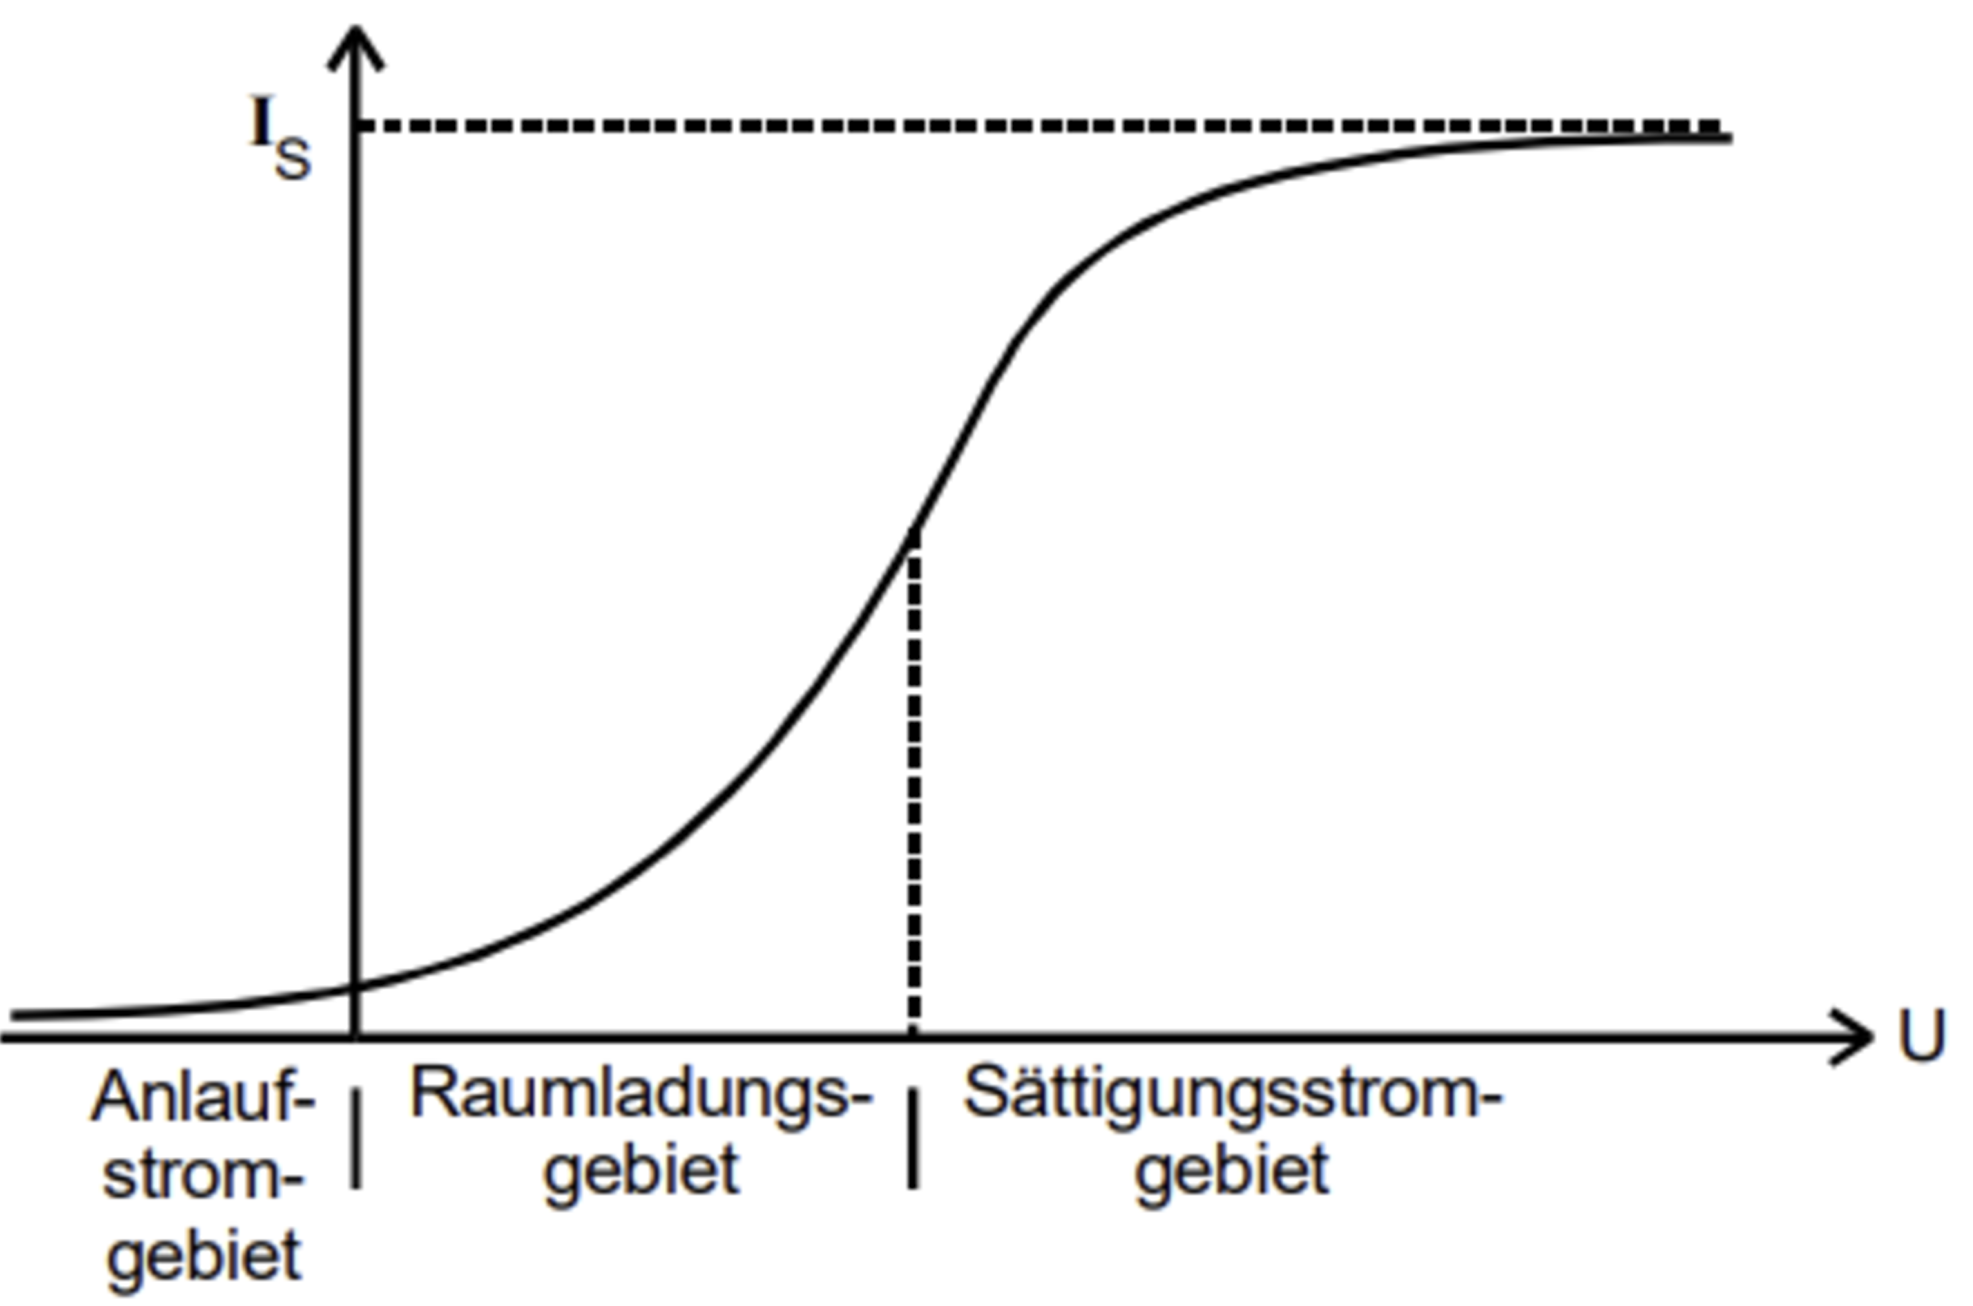
\includegraphics[width=0.9\textwidth]{../build/Kennlinie.pdf}
    \caption{Kennlinie des Geiger-Müller-Zählrohrs.}
\end{figure}

\noindent Die Steigung des Arbeitsplateaus kann auch mithilfe der folgenden Gleichung bestimmt werden.

\begin{equation*}
    s = \frac{z(U_\text{A} + \qty{50}{\volt}) - z(U_\text{A} - \qty{50}{\volt}) } { z(U_\text{A}) } \cdot 100\% / \qty{100}{\volt}.
\end{equation*}

\noindent Dabei ist $z$ die Zählrate bei der jeweiligen Spannung. $U_\text{A}$ ist die Arbeitsspannung, mit der 
das Geiger-Müller-Zählrohr betrieben wird. Diese ist das erste Drittel des Arbeitsplateaus. Sie wird daher 
auf $U_\text{A} = \qty{480}{\volt}$ bestimmt. Da die Zählrate in Spannungsschritten von \qty{20}{\volt} gemessen 
wird, wird die Formel dementsprechend angepasst zu  

\begin{equation*}
    s = \frac{z(U_\text{A} + \qty{60}{\volt}) - z(U_\text{A} - \qty{60}{\volt}) } { z(U_\text{A}) } \cdot 100\% / \qty{120}{\volt}.
\end{equation*}

\noindent Die Steigung kann so auf 

\begin{align*}
    a = \qty{0.038\pm0.001}{\per \volt \per \second} \cdot 100\% / \qty{120}{\volt}
\end{align*}

\noindent bestimmt werden. 


\subsection{Strom des Geiger-Müller-Zählrohres}
\noindent Es soll nun die im Geiger-Müller-Zählrohr erzeugten Ladungen als Funktion der Detektorspannung aufgetragen werden. \\ 
\noindent Dazu wird zunächst der Strom des Messgerätes bei den jeweiligen Spannungen gemessen. Dabei werden folgende Werte notiert:

\begin{table}[H]
    \caption{Messwerte der Spannung und des Stroms auf 120s.}
    \label{tab:Kennlinie}
    \begin{minipage}[t]{0.5\textwidth}
        \vspace{0pt}
        \centering
    \begin{tblr}{
    colspec = {S[table-format=3.0] S[table-format=1.1]},
    row{1} = {guard, mode = math} 
    }
    \toprule
    \text{Spannung} \mathbin{/} \unit{\volt} & \text{Stroms I} \mathbin{/} \qty[per-mode=reciprocal]{}{\micro \ampere} \\
    \midrule
        300 &   0.1     \\
        320 &   0.2     \\
        340 &   0.2     \\
        360 &   0.4     \\
        380 &   0.5     \\
        400 &   0.6     \\
        420 &   0.7     \\
        440 &   0.8     \\
        460 &   1.0     \\
        480 &   1.1     \\
        500 &   1.2     \\
    \end{tblr}
\end{minipage}\hfill
\begin{minipage}[t]{0.5\textwidth}
    \vspace{0pt}
    \centering
    \begin{tblr}{
        colspec = {S[table-format=3.0] S[table-format=1.1]},
        row{1} = {guard, mode = math} 
        }
        \toprule
        \text{Spannung} \mathbin{/} \unit{\volt} & \text{Stroms I} \mathbin{/} \qty[per-mode=reciprocal]{}{\micro \ampere} \\
        \midrule
            520 &   1.3     \\
            540 &   1.4     \\
            560 &   1.7     \\
            580 &   1.6     \\
            600 &   1.8     \\
            620 &   1.9     \\
            640 &   2.0     \\
            660 &   2.0     \\
            680 &   2.0     \\
            700 &   2.2     \\
            720 &   2.4     \\
        \end{tblr}
    \end{minipage}\hfill
\end{table}


\noindent Trägt man nun den gemessenen Strom gegen die Betriebsspannung auf, so entsteht der folgende plot.

\begin{figure}[H]
    \centering
    \includegraphics[width=0.9\textwidth]{../build/Stromstaerke.pdf}
    \caption{Ladungen im Geiger-Müller-Zählrohr bei verschiedenen Betriebsspannungen.}
\end{figure}

\noindent bemerkenswert ist, dass die Kennlinie nicht zu erkennen ist. Der Stromverlauf ist sehr linear.



\subsection{Bestimmung der Totzeit}
\noindent Die Totzeit des Geiger-Müller-Zählrohres kann mithilfe eines Oszilloskops abgelesen werden. 

\begin{figure}[H]
    \centering
    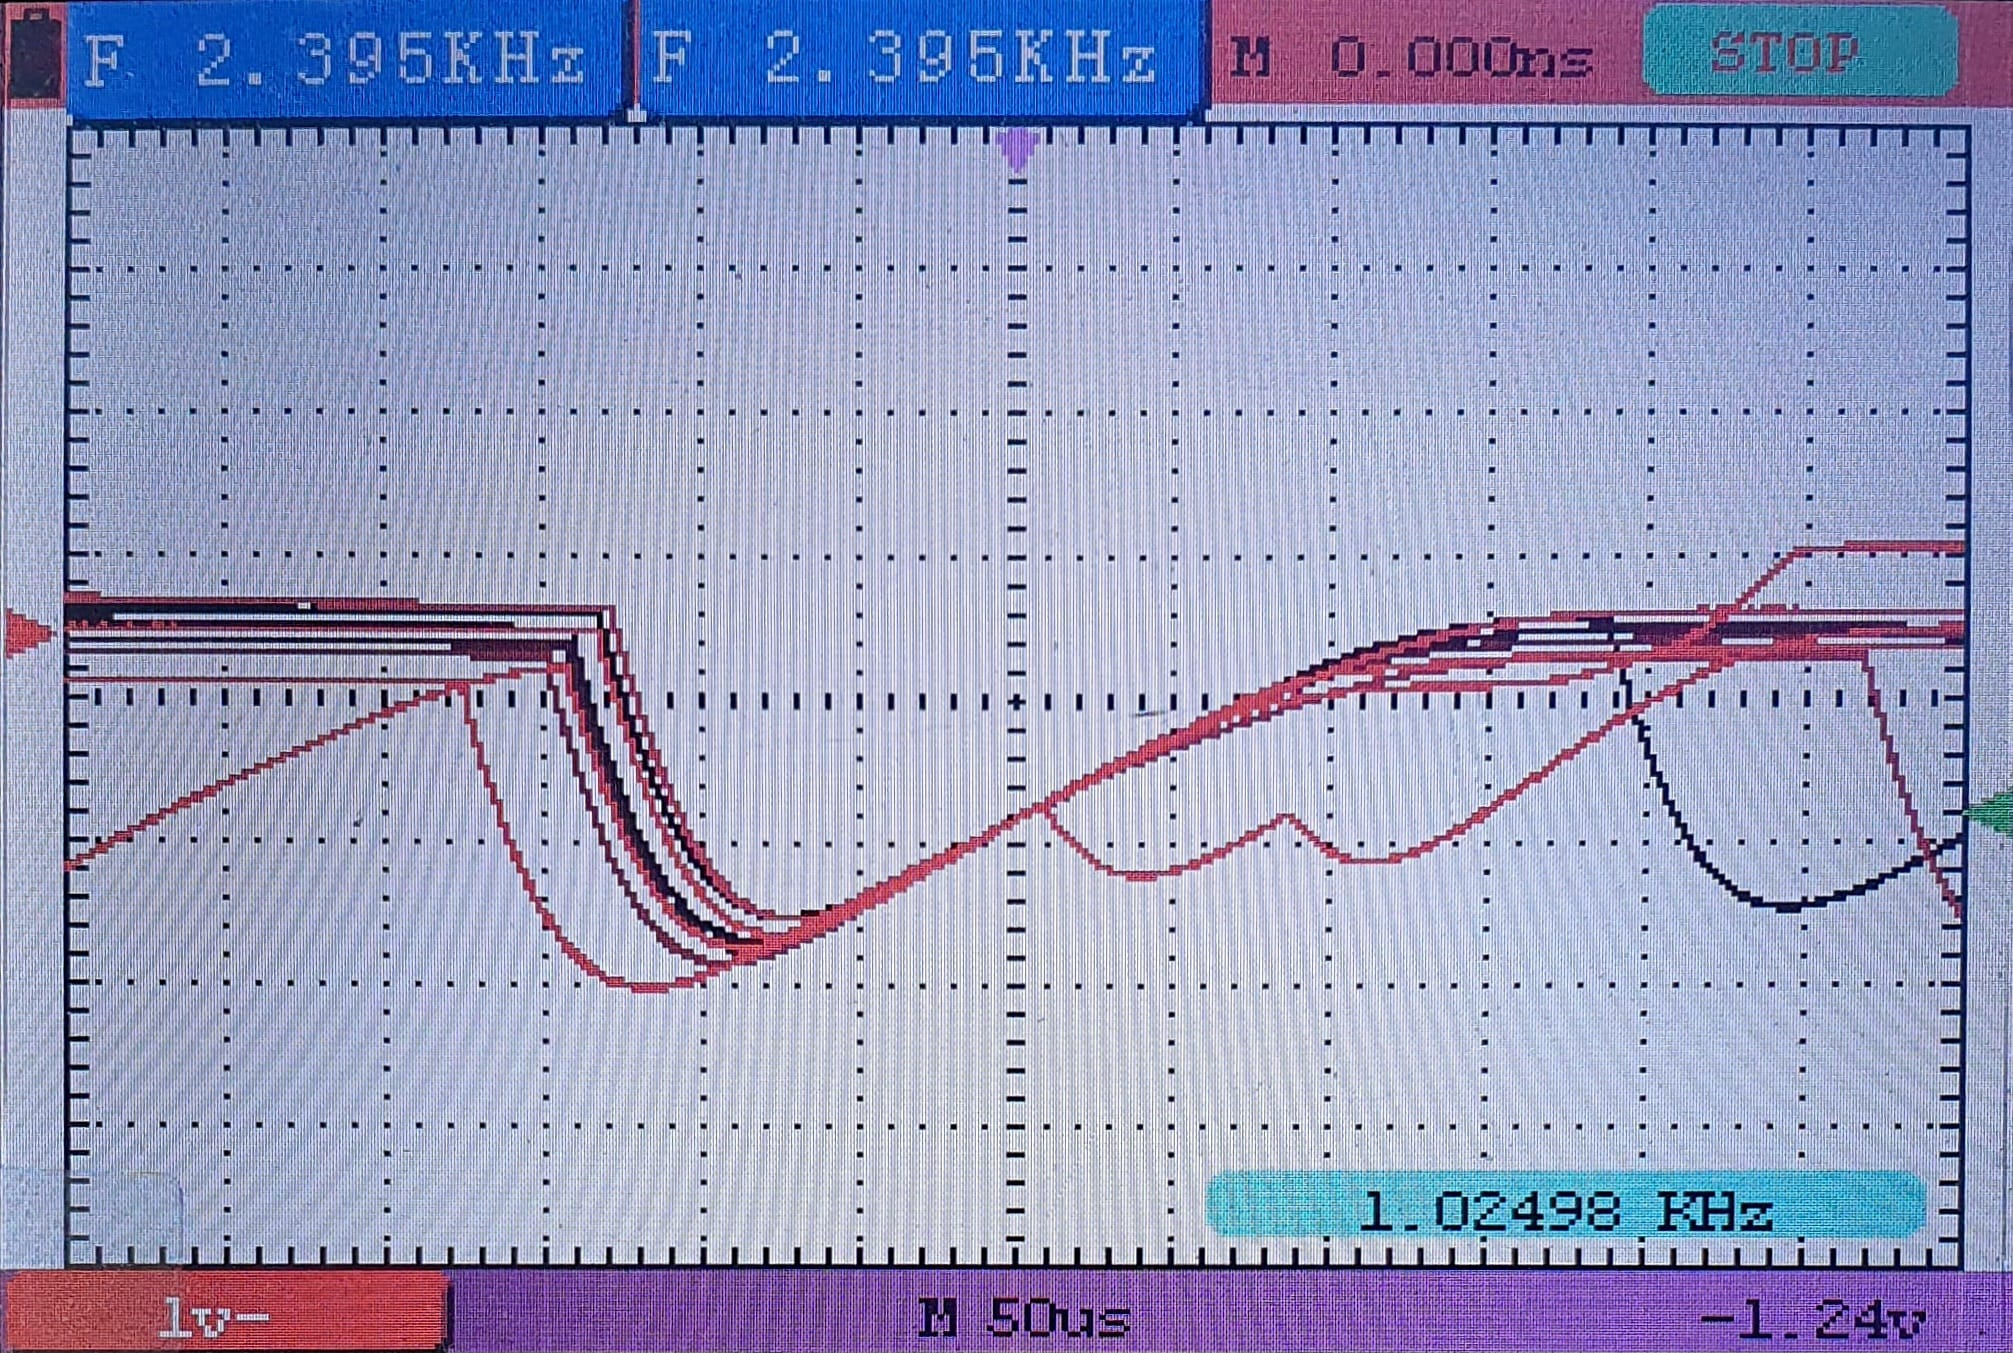
\includegraphics[width=0.9\textwidth]{Oszilloskop.jpg}
    \caption{Totzeit des Geiger-Müller-Zählrohrs am Oszilloskop.}
\end{figure}

\noindent So wird die Totzeit auf 

\begin{align*}
    \tau = \qty{260\pm5}{\micro \second}
\end{align*}

\noindent bestimmt.
Mithilfe der zwei-Quellen-Methode kann die Totzeit über Gleichung \eqref{eqn:Totzeit} bestimmt werden. Die Messergebnisse der drei 
Messungen über $\qty{120}{\second}$ werden nun aufgeführt.

\begin{align*}
    N_{1 } &= \num{154865\pm394}    \\
    N_{2 } &= \num{145314\pm381}    \\
    N_{12} &= \num{258114\pm508}    \\
\end{align*}

\noindent Nun müssen die Messdaten allerdings in SI umgerechnet werden, weshalb durch \qty{120}{\second} geteilt werden muss. 
Dementsprechend wird mit den folgenden Werten gerechnet.

\begin{align*}
    N_{1 } &= \qty[per-mode=reciprocal]{1290.5\pm3.3}{\per\second}    \\
    N_{2 } &= \qty[per-mode=reciprocal]{1211.0\pm3.2}{\per\second}    \\
    N_{12} &= \qty[per-mode=reciprocal]{2151.0\pm4.0}{\per\second}    \\
\end{align*}

\noindent Diese Werte werden nun in Gleichung \eqref{eqn:Totzeit} eingesetzt, um die Totzeit zu berechnen. Dabei wird die Totzeit auf

\begin{align*}
    \tau = \qty{235\pm7}{\micro \second}
\end{align*}

\noindent konstituiert.











\end{document}
